% Revised scientific protocol v2
\documentclass[applsci,article,submit,pdftex,moreauthors]{Definitions/mdpi}

%--------------------------------------------------------------------
% MDPI internal commands - do not modify
%--------------------------------------------------------------------
\firstpage{1}
\makeatletter
\setcounter{page}{\@firstpage}
\makeatother
\pubvolume{1}
\issuenum{1}
\articlenumber{0}
\pubyear{2026}
\copyrightyear{2026}
\datereceived{ }
\dateaccepted{ }
\datepublished{ }
\hreflink{https://doi.org/}
\graphicspath{{figures/}}
\setlength{\headheight}{25pt}

%--------------------------------------------------------------------
% Front matter
%--------------------------------------------------------------------
\Title{Planar Path Synthesis Across Eight Kinematic Models: Search Budget, Closed-Cycle Validity and Quality Diversity}

\TitleCitation{Planar Path Synthesis Across Eight Kinematic Models: Search Budget, Closed-Cycle Validity and Quality Diversity}

\Author{R\'omulo Sandoval Fl\'orez $^{1}$*,
Claudia Patricia Parra Medina $^{2}$ and
Dario Amaya Hurtado $^{2}$}

\AuthorNames{R\'omulo Sandoval Fl\'orez, Claudia Patricia Parra Medina
and Dario Amaya Hurtado}

\AuthorCitation{Sandoval Fl\'orez, R.; Parra Medina, C.P.; Amaya
Hurtado, D.}

\address{%
$^{1}$ \quad Universidad ECCI, Grupo de Investigaci\'on GIDMyM,
Bogot\'a 111311, Colombia; romulo@ecci.edu.co\\
$^{2}$ \quad Universidad Militar Nueva Granada, Grupo de Investigaci\'on
GAV, Bogot\'a 110111, Colombia; claudia.parra@unimilitar.edu.co;
dario.amaya@unimilitar.edu.co}

\corres{Correspondence: romulo@ecci.edu.co}

\usepackage{longtable}
\newcommand{\VTwoRuns}{2880}
\newcommand{\VTwoQDRuns}{240}
\newcommand{\CDGHardCompact}{21}
\newcommand{\CDGHardRelaxed}{19}
\newcommand{\CDGHardQuality}{0}
\abstract{Path-synthesis outcomes depend on the kinematic model, parameter bounds, search policy and validity checks. We compare eight explicit planar models on seven ordered curves at 90 mm width. Graph reconstruction shows that several legacy Watt/Stephenson names do not identify distinct classical inversions. We correct a slider-crank geometry that changes effective rod length and geared-five-bar ratios incompatible with a one-turn state cycle. The revised study includes \VTwoRuns{} model-level searches with exact simulator budgets, independent covariance matrix adaptation evolution strategy (CMA-ES) checks and additional targets, plus \VTwoQDRuns{} matched-budget quality-diversity runs with component and grid controls. On medium-hard, CD-G yields \CDGHardCompact/30 and \CDGHardRelaxed/30 retained strict motion-valid (SMV) designs under compact and relaxed bounds at 20 000 calls. None passes the all-dyad 30-degree transmission screen. Full QD yields 9/30 SMV seeds versus 7/30 for the capped baseline, without a significant adjusted paired difference. Selected-vector checks expose sensitivity to discretization. We release uncertainty estimates, effective bounds, retained vectors and validation scripts. The results characterize recoverability under specified protocols; they do not establish intrinsic family rankings, collision-free packaging or industrial performance.}
\keyword{path synthesis; kinematic validation; mechanism models; stochastic search; simulation budget; quality diversity}
\begin{document}
\section{Introduction}
\linelabel{rev:intro:start}Planar path synthesis combines two decisions: choosing a kinematic model and finding dimensions that reproduce an ordered curve. Classical analytical synthesis establishes useful constructions for specified task positions, while numerical optimization can accommodate dense curves and additional constraints \cite{Freudenstein1954,McCarthy2010,Soh2008,Plecnik2016a}. A stochastic search, however, observes only the part of a parameter space that its operators and computational budget reach. A failed run therefore does not establish that the corresponding mechanism cannot generate the path.

Comparative metaheuristic studies address the performance of optimization procedures for a stated synthesis formulation \cite{Kang2022,Winyangkul2026}. Graph-based approaches can also search the structural design space instead of choosing dimensions within a fixed model \cite{Fogelson2023}. Our study addresses a narrower question: which solutions can be recovered reproducibly from explicitly specified models, boxes of parameters and search procedures? The contribution is a reproducible experimental protocol and a documented correction of several ways in which a capability comparison can overstate its evidence. It is not a new universal optimizer or an exhaustive classification of mechanism architectures.

The distinction between a model and a classical family is essential here. The initial implementation used the identifiers \texttt{wattI}, \texttt{wattII} and \texttt{stephensonI/II/III}. Reconstructing their body--joint graphs showed that these names do not correspond to five distinct classical six-bar inversions. We retain the identifiers in the data for traceability, but use explicit model labels in the revised comparison. We also distinguish geometric fitting from a physically repeatable cycle and from acceptable transmission quality. These corrections change the interpretation of several originally reported successes.

The experiments extend the original three analytic paths with four geometrically different targets, including a published mathematical reference curve and a published engineering-reference contour. A factorial study varies target, parameter-bound profile and cumulative simulation budget separately. An independent CMA-ES implementation checks whether conclusions depend on the hybrid search. A controlled quality-diversity (QD) study separates MAP-Elites selection from surrogate-guided mutation and tests grid resolution. Every main cell has 30 seeds and every counted search evaluation, including failed closures and local-refinement calls, consumes the stated budget.\linelabel{rev:intro:end}

\section{Materials and Methods}
\subsection{Model identity and geometry}\label{sec:models}
\linelabel{rev:models:start}Table~\ref{tab:v2_models} defines the eight models and their relation to the legacy identifiers. The input angle increases over one complete turn. Except for the translated slider model, $O_2=(0,0)$ and $O_4=(L_0,0)$, with $L_1$ replacing $L_0$ in the four-bar. The first loop of the six-bar models is $O_2$--$A$--$B$--$O_4$. A tracer offset is rigidly attached to a specified link; it is not an additional joint or degree of freedom. Appendix~\ref{app:bounds} gives all effective compact and relaxed bounds.

\begin{table}[H]
\caption{Explicit kinematic models. Legacy identifiers are software labels, not a claim of eight distinct classical families. Tracer definitions and all bounds are provided in Methods and the appendix.}
\label{tab:v2_models}
\centering
\small
\begin{tabular}{@{}lllp{5.1cm}@{}}
\toprule
Model & Legacy ID & Parameters & Construction \\
\midrule
F4 & fourbar & 6 & One loop; tracer fixed to AB \\
SC & slidercrank & 5 stored; 4 shape & Crank--slider; tracer on AB \\
CD-G & wattI & 12 & C fixed to AB; second dyad C-D-G \\
RC-G & wattII & 12 & C fixed to rocker; second dyad C-D-G \\
A-O4 & stephensonI & 8 & Second dyad A-D-O4 \\
B-O2 & stephensonII & 8 & Second dyad B-D-O2 \\
C-O4 & stephensonIII & 10 & C fixed to AB; second dyad C-D-O4 \\
G5 & gearedFiveBar & 8 real + ratio & Two driven cranks; closure at C \\
\bottomrule
\end{tabular}
\end{table}


Watt chains have adjacent ternary bodies, whereas Stephenson chains have their ternary bodies separated by binary bodies \cite{Plecnik2016b}. In CD-G, ground and coupler $AB$ are the nonadjacent ternary bodies. In RC-G, ground and the rocker carrying $C$ are adjacent ternary bodies. The other three six-bar implementations contain coincident-joint specializations. In particular, C-O4 is the CD-G construction with $G=O_4$. In A-O4 the tracer is determined by subloop $O_2$--$A$--$D$--$O_4$; its additional loop restricts feasibility without independently determining the tracer. Thus these eight rows are not eight disjoint classical families, and differences between them include tracer placement, parameterization and bounds.

Loop closure is evaluated by circle intersections, selecting the initial assembly branch explicitly and following the nearest intersection at subsequent input angles. Impossible intersections and degenerate direction vectors are invalid evaluations. For SC, the corrected geometry is
\begin{align}
 O&=(x_0,0),& A&=O+r(\cos\theta,\sin\theta),\\
 B&=(A_x+\sqrt{\ell^2-A_y^2},0),&
 P&=A+q\ell\,\mathbf u_{AB}+h\,\mathbf v_{AB}.
\end{align}
This keeps $|AB|=\ell$. The historical implementation added $x_0$ to $B$ without translating $A$, and therefore generally changed the effective rod length during motion. Here $x_0$ is a rigid translation and is unidentifiable under the pose-invariant metric; SC has five stored parameters but only four affect its curve shape. Its bound is retained for traceability rather than counted as an independent shape variable.

For G5, $B=O_4+L_4[\cos(\rho\theta+\phi),\sin(\rho\theta+\phi)]$. A continuous $\rho$ generally does not return $B$ to its initial position after one input turn: the endpoint separation is $2L_4|\sin(\pi\rho)|$. The revised one-turn experiment uses $\rho\in\{-3,-2,-1,1,2,3\}$. The nearest admissible ratio is used and the actual simulated vector is archived. This is a mixed discrete--continuous model with eight real variables and one categorical ratio. Other rational ratios would require evaluating a stated common multi-turn period and are outside this experiment.

The profiles are boxes of design parameters, not occupied-envelope constraints. Compact/relaxed secondary-link limits are 180/260~mm, including the corrected SC rod; ground distances and tracer offsets also change according to the full bounds table. Neither profile imposes a collision-free envelope, a fixed absolute curve placement or a fabrication certificate.
For a descriptive geometric check, Appendix~\ref{app:envelopes} reports the sampled axis-aligned envelope of all represented kinematic points, including fixed anchors and the tracer, at 1920 input intervals for minimum-RMS designs selected at 20\,000 calls. Its area is $(x_{\max}-x_{\min})(y_{\max}-y_{\min})$; the maximum radius is measured from $O_2$, or the translated crank anchor $O$ for SC. Dense closure failures retain their counts and have no envelope statistic. This post-hoc point measure is not a search constraint and does not include unmodeled body thickness or collision clearance.\linelabel{rev:models:end}

\subsection{Targets and geometric error}\label{sec:targets}
\linelabel{rev:targets:start}The easy, medium and medium-hard targets are independent analytic Fourier curves, not outputs of a benchmarked model. Their formulas and normalization are released in the code. The original 120-point versions are kept fixed for the corresponding search comparisons. The additional targets are the Bernoulli lemniscate, a superellipse with exponent four and an asymmetric curve with an inward harmonic deformation. The lemniscate is a published mathematical reference \cite{BernoulliReference}; it is not a measured industrial path. The other two are specified analytic tests. None is selected from the evaluation outcomes.

The seventh target is the altered sharp-trailing-edge NACA0012 contour published by the NASA-linked Turbulence Modeling Resource \cite{NASATMR}. We archive all 12\,299 supplied coordinates and their SHA-256 digest. Preprocessing discards the zero third coordinate, preserves contour order, resamples the closed curve by arc length, centers it and normalizes its width to 90~mm, without smoothing. This adds an externally specified engineering-reference geometry; it is not a measured mechanism trajectory or evidence of application performance. Its separate protocol was fixed before running its 30 seeds per model.

\begin{table}[H]
\caption{Descriptive geometry of 960-point closed target polygons at 90 mm width. Length and absolute turning are polygonal approximations. These descriptors are not a universal difficulty score; the ordered Bernoulli path additionally has a self-intersection.}
\label{tab:v2_descriptors}
\centering
\small
\begin{tabular}{@{}lrrr@{}}
\toprule
Target & Height mm & Length mm & Absolute turn rad \\
\midrule
Easy & 50.11 & 224.80 & 6.28 \\
Medium & 69.42 & 259.36 & 7.98 \\
Medium-hard & 63.49 & 269.17 & 8.20 \\
Bernoulli & 31.82 & 235.98 & 9.42 \\
Rectangle & 58.50 & 261.82 & 6.28 \\
Asymmetric & 53.30 & 218.72 & 9.32 \\
NACA0012 & 10.71 & 183.52 & 6.28 \\
\bottomrule
\end{tabular}
\end{table}


\begin{figure}[H]
\centering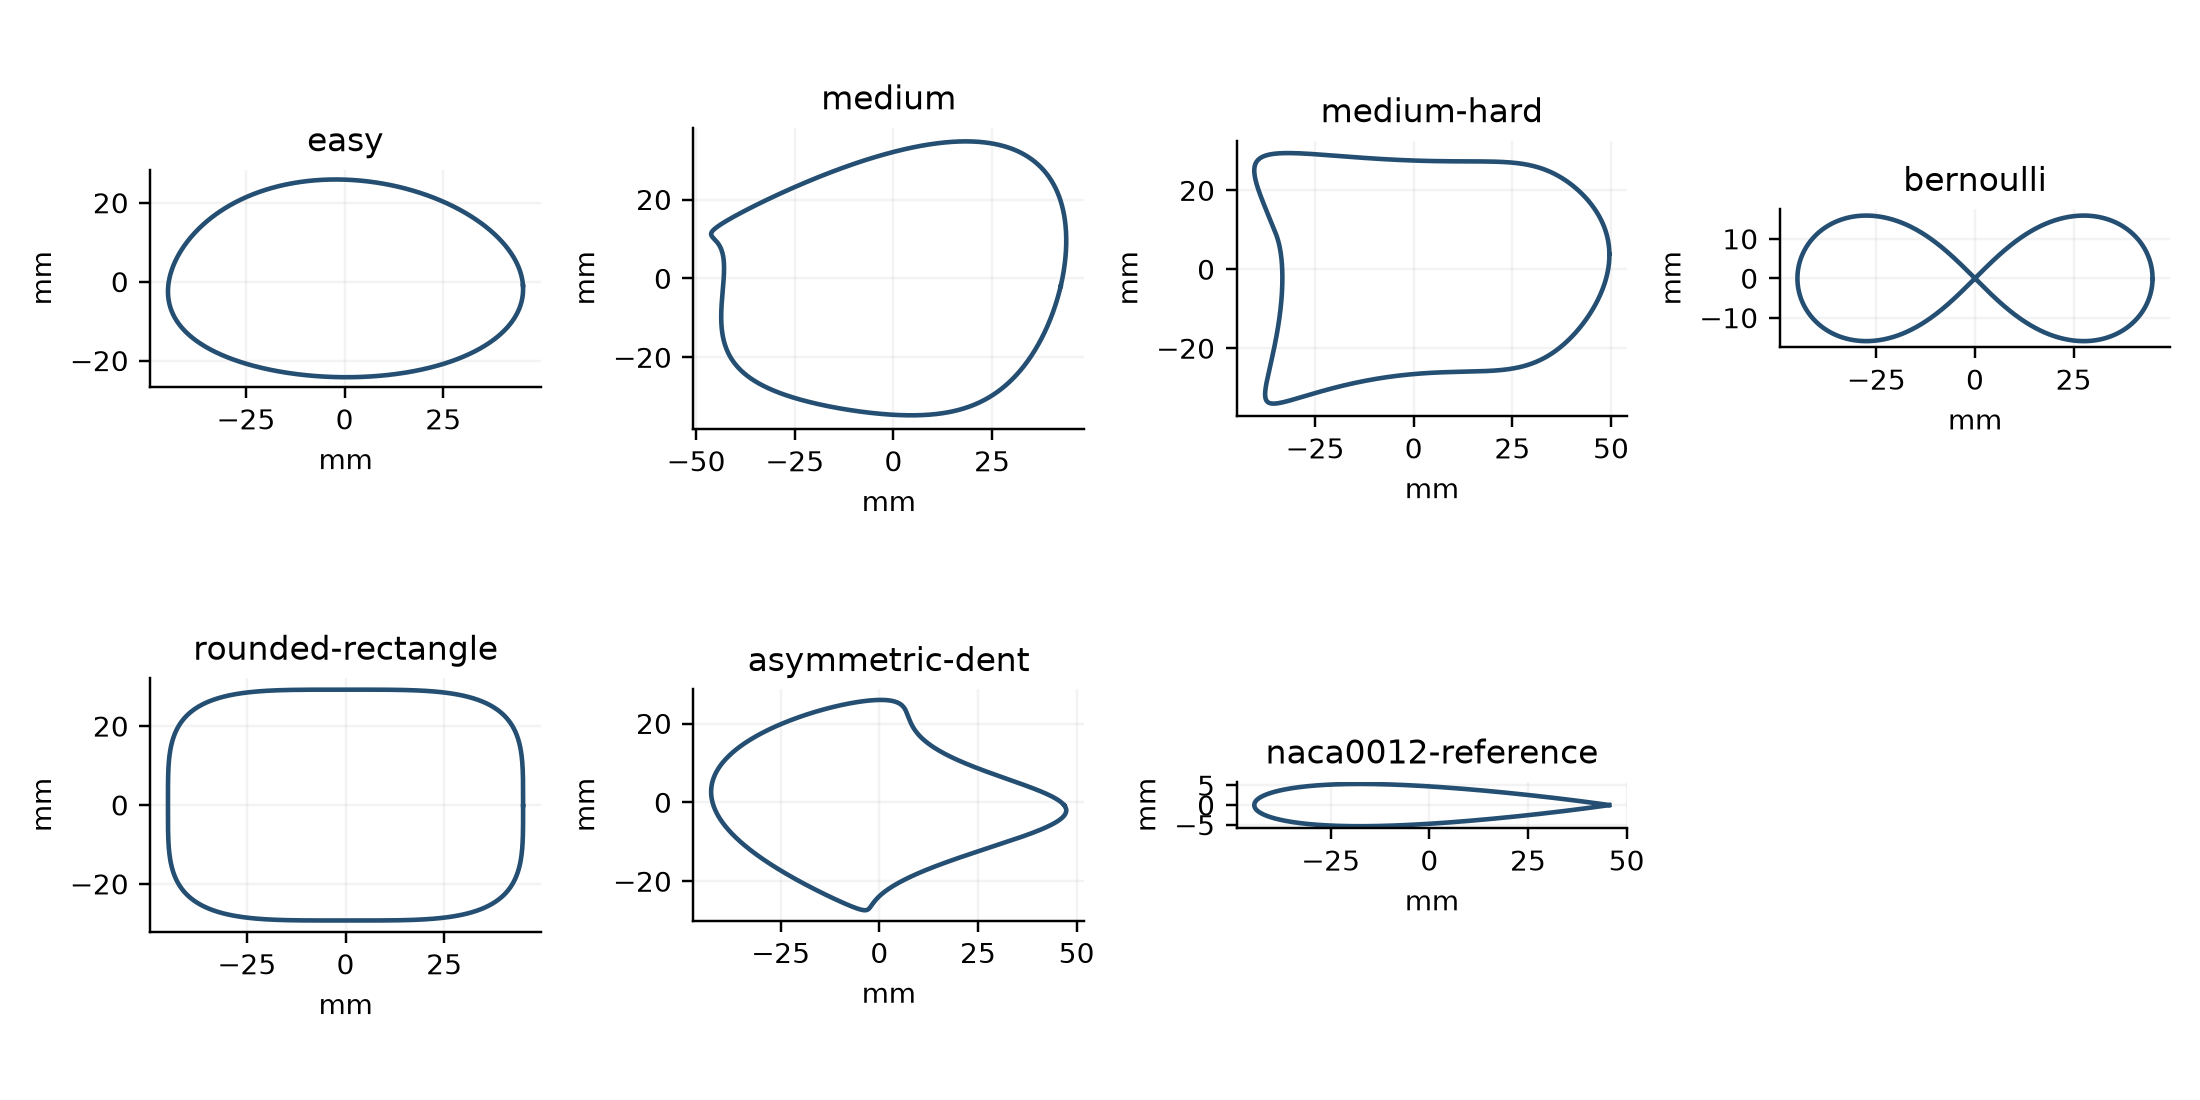
\includegraphics[width=\textwidth]{v2_targets.png}
\caption{The seven target curves, normalized to 90~mm width. Names such as medium-hard denote the original test cases; geometric descriptors are not universal measures of synthesis difficulty. The ordered lemniscate contains a self-intersection. NACA0012 is prescribed engineering-reference geometry.}\label{fig:v2_targets}
\end{figure}

Both target and generated paths are sampled approximately uniformly in arc length. For an ordered generated path $P$ and target $Y$, the metric minimizes over a proper planar rotation, translation and cyclic index shift:
\begin{equation}
 E_{\rm RMS}=\min_{R\in SO(2),\,t,\,k}
 \sqrt{N^{-1}\sum_{i=1}^{N}\|RP_i+t-Y_{i-k}\|^2}.
\end{equation}
$E_{\max}$ is the largest point error at the alignment selected by RMS. Reflection and order reversal are not permitted. The metric preserves cyclic point order but deliberately ignores absolute pose, input timing and dwell requirements. Consequently, a low fitting error alone is insufficient for an application requiring fixed placement or a prescribed speed law.

Accuracy-strict means $E_{\rm RMS}\leq1$~mm and $E_{\max}\leq2$~mm. These are operational criteria at 90~mm path width, not validated industrial tolerances or guarantees of manufacturing precision. The supplement recomputes selected-design results over RMS limits 0.5, 1, 1.5 and 2~mm and maximum-error limits 1, 2, 3 and 4~mm. This post-hoc sensitivity keeps the selected vector fixed; it is distinguished from the search-success indicator based on any evaluated candidate.\linelabel{rev:targets:end}

\subsection{Cycle and transmission checks}\label{sec:validation}
\linelabel{rev:validation:start}Every retained design is checked over the input cycle with the endpoint $2\pi$ included. The checks evaluate closure residuals for every rigid link, return of all moving joints and tracer to their initial state, and nonzero loop-orientation signs without sampled branch changes. A motion-valid result requires endpoint and link residuals no larger than $10^{-6}$~mm and consistent oriented-loop signs. Tests use 120, 480 and 1920 intervals for archived selected designs; the revised searches retain a 1920-interval check and a separate error-resolution analysis. The fitting resolution $N$ and the motion-check interval count are distinct uses of sampling density: $N=120$, 480 or 960 governs the arc-length comparison of a selected curve against the target, whereas the 1920-interval check traces the returned mechanism over its input cycle. These are explicit dense numerical checks, not a proof excluding an unsampled defect.

For every solved revolute dyad the transmission measure is the acute angle $\arccos(|\mathbf u\cdot\mathbf v|/(\|\mathbf u\|\|\mathbf v\|))$, which detects approach to either 0 or 180 degrees. All relevant dyads are included. For SC the measure is 90 degrees minus connecting-rod obliquity to the sliding direction. A separate quality indicator requires a minimum of 30 degrees. That cutoff is a declared design screen, not a universal feasibility law. A design can therefore pass accuracy and complete the cycle while failing the transmission-quality screen.

The historical G5 successes with noninteger ratios are not counted as repeatable one-turn mechanisms. Historical SC designs with variable effective rod length are likewise excluded from validated motion rates. Original numerical outputs are preserved as protocol-specific fitting results rather than silently replaced.\linelabel{rev:validation:end}

\subsection{Search and exact computational budget}\label{sec:search}
\linelabel{rev:search:start}The hybrid procedure combines Latin-hypercube samples, shape templates, neighborhoods around elites, differential evolution, diverse candidate selection, Powell refinement and bounded least-squares polishing \cite{Storn1997,Virtanen2020}. The scalar search cost retains the historical weights 1, 0.22, 0.03, 0.08 and 0.015 on RMS, maximum error, smoothness, a loop-margin penalty and a size penalty, respectively. The margin penalty is a heuristic soft term; it is not used as a substitute for the cycle and transmission checks. A controlled run removes its contribution from both scalar cost and the least-squares residual.

Equal settings are not equal computation. In the implementation of differential evolution, population size scales with the number of free variables, so fixed iteration and population-multiplier settings do not equalize simulator calls \cite{SciPyDE}. We therefore instrument the simulator itself. Every call counts, including invalid states and finite-difference evaluations during local refinement. Search is interrupted at the exact limit, retaining only candidates actually evaluated; unfinished polishing is not completed outside the budget. Tracking and subsequent validation do not propose new search candidates.

The factorial study uses 8 models, 2 targets (medium and medium-hard), 2 bound profiles and 30 seeds, giving 960 searches. Each has 40\,000 calls with cumulative checkpoints at 10\,000, 20\,000 and 40\,000. These are dependent checkpoints of the same trajectory, not independent restarted searches or extra replicates. When the hybrid routine terminates naturally before the limit, it restarts with the remaining seeded random stream. The search parameters and restart rule are frozen in the protocol and archived code. Post-hoc verification is outside the search budget and is not fed back into either optimizer.
Table~\ref{tab:v3_campaigns} reconciles the 2880 model-level searches. The separate repetition, recovery and multi-model QD runs are not included in that total.
\begin{table}[H]
\caption{Campaign inventory. The factorial checkpoints reuse the same searches and are not additional independent runs. The 1200-target block comprises five separate 240-run campaigns. Every numerical budget counts simulator invocations, including invalid states and refinement.}
\label{tab:v3_campaigns}
\centering
\small
\begin{tabular}{@{}p{9.0cm}rr@{}}
\toprule
Campaign & Runs & Calls per run \\
\midrule
Factorial: 8 models $\times$ 2 targets $\times$ 2 profiles $\times$ 30 seeds & 960 & 40 000 \\
Independent CMA-ES: 8 $\times$ 2 $\times$ 30 & 480 & 20 000 \\
Easy + 3 new analytic + NACA0012: 8 $\times$ 5 $\times$ 30 & 1200 & 20 000 \\
Penalty ablation without singularity term: 8 $\times$ 30 & 240 & 20 000 \\
\textbf{Main model-level total} & \textbf{2880} &  \\
Additional repetition batches (separate) & 60 & 20 000 \\
Own-curve diagnostic searches (separate) & 8 & 80 000 \\
Multi-model QD policy/grid runs (separate) & 240 & 40 000 total \\
\bottomrule
\end{tabular}
\end{table}


The independent comparison uses the official pycma implementation \cite{HansenCMA} with normalized box coordinates, random initial means and an initial step size of 0.25. It uses the same corrected simulator, objective and bounds, but none of the hybrid shape templates. It runs both medium targets under compact bounds with 30 seeds and exactly 20\,000 calls per model/seed. Discrete G5 ratios use the same projection for both optimizers. Easy and the four additional targets use compact bounds and 20\,000 calls with 30 seeds per model. Two additional 30-seed batches repeat CD-G/medium/compact at the base budget to describe between-batch variability without confusing it with a change of protocol.\linelabel{rev:search:end}

\subsection{Controlled quality-diversity experiment}\label{sec:qd}
\linelabel{rev:qd:start}MAP-Elites retains high-performing solutions across a chosen descriptor space \cite{Mouret2015,Pugh2016}. We use the original interpretable descriptors: curve elongation from the covariance eigenvalues and the logarithm of a discrete turning-energy measure. Their ranges are frozen from the separate historical pilot; clipping at these ranges is a limitation of the diversity metric. Descriptor-space coverage does not certify mechanical diversity.

The revised component experiment is MAP-Elites present/absent crossed with local surrogate guidance present/absent. Without MAP-Elites, a bounded global elite set of 576 vectors replaces the niche archive. With MAP-Elites, parents are selected uniformly from occupied niches. The surrogate is the original local weighted ridge model fitted to 30 neighbors in normalized parameters, used for half the mutations after sufficient family-specific observations. Gaussian mutation, 5\% immigration, initialization, shared cross-model archive policy and the corrected simulator remain fixed. Differential evolution is disabled throughout these component arms.

Each run uses 24\,000 search calls and 16\,000 refinement calls, the latter allocated equally across models. A separate capped hybrid baseline uses 5000 calls per model, with the historical QD baseline settings and no DE. All five arms therefore use exactly 40\,000 calls, including refinement, and 30 seeds. This capped baseline is explicitly different from the original baseline with a natural, variable total.

The full MAP-Elites-plus-surrogate arm is additionally evaluated on native grids with 12, 18 and 36 cells per side; the 24-grid arm is reused from the two-by-two component study without being counted twice. Coverage and QD-score always use the same 24-by-24 reference grid. Thus a change in native resolution is not rewarded merely for changing the denominator of the reported coverage. Vectors of retained strict elites are saved in every arm for symmetric post-hoc checks.
Coverage is the fraction of the 576 reference cells occupied by a valid evaluated design; QD-score sums $(5-\min(E_{\rm RMS},5))/5$ over the minimum-RMS design in each occupied cell. These descriptors and scores are based on fitted curves before the separate motion/transmission filters, so occupancy does not imply strict or quality-valid recovery.\linelabel{rev:qd:end}

\subsection{Statistics and reproducibility}\label{sec:statistics}
\linelabel{rev:statistics:start}The experimental unit is a seed within a specified target/model/profile/policy cell. Rates are reported as counts out of 30 with marginal Wilson 95\% intervals \cite{Wilson1927}. Common seed labels define blocks for the revised profile contrasts; they do not make different historical configurations causally interchangeable. Compact-minus-relaxed RMS differences are summarized with paired shifts and bootstrap intervals; paired strict indicators use exact McNemar tests \cite{McNemar1947}. RMS and indicator contrasts form separate multiplicity families across the two targets and eight models, each adjusted by Holm \cite{Holm1979}. Cumulative budget checkpoints are described as repeated observations, not pooled into a larger sample size.

We recomputed the historical effect sizes independently. The paired rank-biserial effect is $(W_+-W_-)/(W_++W_-)$. For the historical CD-G bound comparison it is 0.501, and for historical G5 it is $-0.200$. The raw CD-G RMS $p=0.01546$ becomes 0.09276 in the six-contrast family defined for that retrospective analysis. The observed strict discordances are 11 and 5, giving exact McNemar $p=0.2101$; the marginal difference of six successes is not six total discordances. Exact power sensitivity under an assumed total discordance probability of $16/30$ gives approximately 24.7\% power for a 0.20 difference at unadjusted $\alpha=0.05$. About 0.374 difference is needed for 80\% power under those assumptions, or about 0.439 with a conservative $0.05/6$ threshold. These are assumption-dependent calculations, not post-hoc evidence of equivalence.

The original QD baseline retains the strict archive, and seed success requires at least one accuracy-strict elite in that archive. An earlier reanalysis incorrectly used the three-seed pilot arm and a missing Boolean field. The repaired counts are 9/15, 10/15 and 10/15 for the original strict baseline, the extended-budget arm and the matched-budget arm; the correct pairing of the original strict baseline with the matched-budget arm has six gains and five losses, $p=1$. These results are retained only as historical precision results, not merged with the corrected 30-seed study.

The release includes effective parameter boxes, actual vectors, target formulas, package versions, source hashes and per-run simulation counts. A compiled double-precision kernel was checked against the unmodified historical geometry in 800 random cases; maximum point and metric differences were below $2\times10^{-13}$~mm. Three model/seed configurations were each repeated three times with identical numerical results. The pilot and determinism seeds are disjoint from the evaluation seeds. The archived recovery tests include a known feasible generator and a separate inverse search that is not given that generator.\linelabel{rev:statistics:end}

\section{Results}
\subsection{What the archived successes establish}\label{sec:historical}
\linelabel{rev:historical:start}The archived medium all-model campaign produced 16 strict CD-G designs out of 30. All 16 retained designs pass the dense sampled cycle checks, but none keeps the 30-degree screen across all relevant dyads. The previous 3/30 recheck included only the first four-bar loop and did not use the acute-angle definition. This does not negate the fitting result; it changes its mechanical interpretation. Historical G5 designs with noninteger transmission ratios do not return their full state after the single evaluated input turn, and the SC offset implementation does not preserve the declared rod length.

The two historical medium campaigns are not replications of an identical protocol: their DE settings, topology order and random-stream consumption differ. Their 7/30 versus 16/30 CD-G results therefore mix changes in search and stochastic variation. The revised comparison uses one controlled design; Table~\ref{tab:v2_repetition} reports three independent base-budget batches under that design. No ranking or uncertainty estimate is obtained by pooling incompatible campaigns.

\begin{table}[H]
\caption{Independent batches of CD-G/medium/compact under the same corrected 20 000-call protocol. Batch 0 uses seeds 1--30; batches 1 and 2 use 1001--1030 and 2001--2030. Main-cell counts are not inflated by pooling these diagnostic repeats. M: retained SMV; intervals are Wilson 95 percent.}
\label{tab:v2_repetition}
\centering
\small
\begin{tabular}{@{}lrrrr@{}}
\toprule
Batch & n & M & CI & Median RMS mm \\
\midrule
0 & 30 & 5 & [0.07, 0.34] & 1.007 \\
1 & 30 & 8 & [0.14, 0.44] & 1.099 \\
2 & 30 & 10 & [0.19, 0.51] & 1.050 \\
\bottomrule
\end{tabular}
\end{table}

An exploratory Pearson homogeneity test of the three independent batches, with success/failure rows $(5,25)$, $(8,22)$ and $(10,20)$, gives $\chi^2=2.219$, two degrees of freedom and $p=0.3297$; the minimum expected cell count is 7.67. This diagnostic does not establish identical recovery rates or zero between-batch variability.\linelabel{rev:historical:end}

\subsection{Factorial target, profile and budget comparison}\label{sec:factorial_results}
\linelabel{rev:factorial:start}Tables~\ref{tab:v2_medium} and \ref{tab:v2_mediumhard} report base-budget results separately for precision, sampled cycle validity and transmission quality. CD-G gives \CDGHardCompact/30 retained SMV designs on medium-hard/compact and \CDGHardRelaxed/30 on medium-hard/relaxed; \CDGHardQuality/30 of the compact designs also pass the transmission screen. The full intervals, parameter vectors and paired contrasts are provided in the supplement. All zero cells retain their denominator; they are not interpreted as impossibility statements.

\begin{table}[H]
\caption{Medium target at 20 000 simulator calls, 30 seeds per model/profile. A: any evaluated accuracy-strict candidate; M: retained strict candidate also passes sampled full-cycle motion checks; Q: that candidate additionally keeps all relevant transmission angles at least 30 degrees. RMS medians refer to minimum-RMS selected designs. C/R denote compact/relaxed. Full Wilson intervals are supplied in the machine-readable supplement.}
\label{tab:v2_medium}
\centering
\small
\begin{tabular}{@{}lrrrrrrrr@{}}
\toprule
Model & A C & M C & Q C & A R & M R & Q R & RMS C & RMS R \\
\midrule
F4 & 0 & 0 & 0 & 0 & 0 & 0 & 1.315 & 1.369 \\
SC & 0 & 0 & 0 & 0 & 0 & 0 & 1.657 & 1.657 \\
CD-G & 5 & 5 & 0 & 17 & 17 & 0 & 1.007 & 0.708 \\
RC-G & 0 & 0 & 0 & 0 & 0 & 0 & 1.396 & 1.355 \\
A-O4 & 0 & 0 & 0 & 0 & 0 & 0 & 1.375 & 1.364 \\
B-O2 & 0 & 0 & 0 & 0 & 0 & 0 & 1.853 & 3.009 \\
C-O4 & 0 & 0 & 0 & 0 & 0 & 0 & 1.277 & 1.265 \\
G5 & 0 & 0 & 0 & 0 & 0 & 0 & 1.292 & 1.281 \\
\bottomrule
\end{tabular}
\end{table}

\begin{table}[H]
\caption{medium-hard target at 20 000 simulator calls, 30 seeds per model/profile. A: any evaluated accuracy-strict candidate; M: retained strict candidate also passes sampled full-cycle motion checks; Q: that candidate additionally keeps all relevant transmission angles at least 30 degrees. RMS medians refer to minimum-RMS selected designs. C/R denote compact/relaxed. Full Wilson intervals are supplied in the machine-readable supplement.}
\label{tab:v2_mediumhard}
\centering
\small
\begin{tabular}{@{}lrrrrrrrr@{}}
\toprule
Model & A C & M C & Q C & A R & M R & Q R & RMS C & RMS R \\
\midrule
F4 & 0 & 0 & 0 & 0 & 0 & 0 & 4.708 & 5.045 \\
SC & 0 & 0 & 0 & 0 & 0 & 0 & 4.674 & 4.676 \\
CD-G & 21 & 21 & 0 & 19 & 19 & 0 & 0.714 & 0.680 \\
RC-G & 0 & 0 & 0 & 0 & 0 & 0 & 5.273 & 5.281 \\
A-O4 & 0 & 0 & 0 & 0 & 0 & 0 & 4.987 & 4.971 \\
B-O2 & 0 & 0 & 0 & 0 & 0 & 0 & 6.013 & 7.024 \\
C-O4 & 0 & 0 & 0 & 0 & 0 & 0 & 2.825 & 2.592 \\
G5 & 0 & 0 & 0 & 0 & 0 & 0 & 1.876 & 1.881 \\
\bottomrule
\end{tabular}
\end{table}


For CD-G/medium, compact and relaxed profiles yield 5/30 and 17/30 retained SMV designs. There is one compact-only and 13 relaxed-only paired success, giving exact McNemar $p=0.001831$ and Holm-adjusted $p=0.02930$ across the 16 profile contrasts. The mean compact-minus-relaxed RMS difference is 0.305~mm (marginal bootstrap 95\% interval 0.160--0.450~mm; Holm-adjusted signed-rank $p=0.004829$). For medium-hard the paired success discordances are eight and six, with adjusted $p=1$; the corresponding mean RMS interval includes zero ($-0.350$ to 0.689~mm). This contrast is target-specific and does not justify a universal claim about relaxed bounds.

\begin{figure}[H]
\centering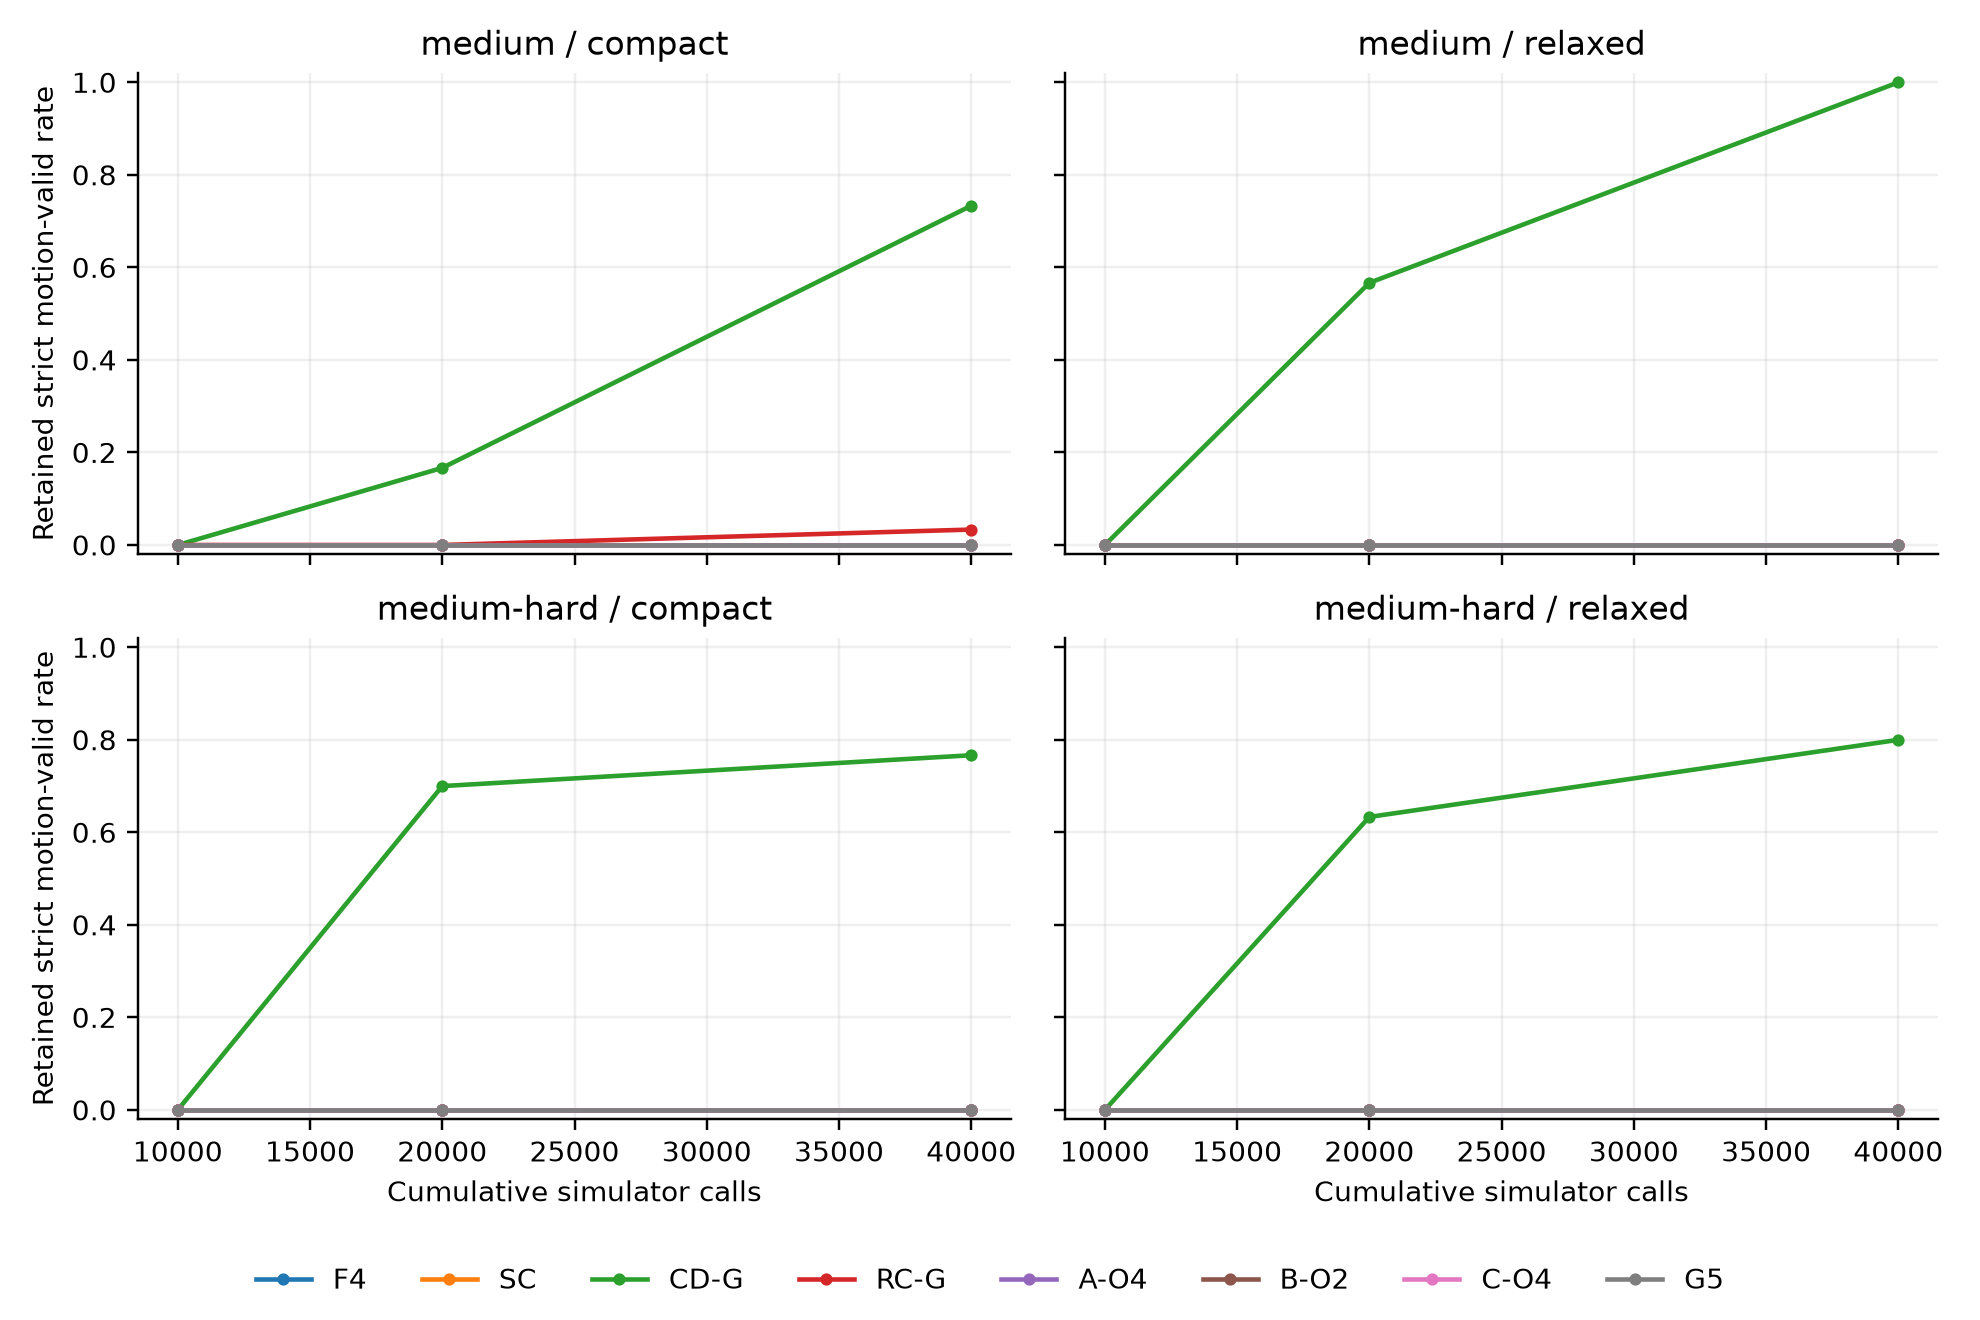
\includegraphics[width=\textwidth]{v2_budget.png}
\caption{Cumulative-budget comparison within the same 30 searches per cell. The indicator refers to the retained strict candidate passing the sampled motion checks. Checkpoints are dependent. Model labels are defined in Table~\ref{tab:v2_models}.}\label{fig:v2_budget}
\end{figure}

The curves in Figure~\ref{fig:v2_budget} make the budget dependence visible without changing target and profile at the same time. A larger parameter box is not a controlled change in occupied envelope, and can also change how effectively a fixed search explores the box. For orientation, concrete CD-G counts from these dependent checkpoints are: medium/compact 0/30, 5/30 and 22/30 at 10 000, 20 000 and 40 000 calls; medium/relaxed 0/30, 17/30 and 30/30; medium-hard/compact 0/30, 21/30 and 23/30; and medium-hard/relaxed 0/30, 19/30 and 24/30. Between the two later checkpoints the medium/compact rate rises from 0.17 to 0.73, whereas medium-hard/compact moves only from 0.70 to 0.77, so the budget response is target- and profile-specific. Consequently, a weak change in aggregate success across profiles does not identify an intrinsic kinematic bottleneck or establish equivalence of profiles.\linelabel{rev:factorial:end}

\subsection{Independent policy and additional paths}\label{sec:independent_results}
\linelabel{rev:independent:start}Table~\ref{tab:v2_independent} compares the hybrid and independent CMA-ES procedures at identical simulator limits. Agreement or disagreement is specific to the model, target and budget, rather than evidence of a universal optimizer ranking. Table~\ref{tab:v2_targets} extends the path set to include different geometric structure and an ordered self-intersection. The associated discretization and tolerance sensitivities hold each selected vector fixed and retain invalid dense-grid designs as failures.

\begin{table}[H]
\caption{Independent optimizer comparison under compact bounds and exactly 20 000 simulator calls per model/seed. The first four numerical columns refer to medium, the last four to medium-hard. M-hyb and M-CMA count retained strict designs passing full-cycle checks for the hybrid engine and for official pycma, respectively; RMS-hyb and RMS-CMA are the corresponding median RMS errors. RMS is in mm.}
\label{tab:v2_independent}
\centering
\small
\setlength{\tabcolsep}{4.5pt}
\begin{tabular}{@{}lrrrrrrrr@{}}
\toprule
& \multicolumn{4}{c}{Medium} & \multicolumn{4}{c}{Medium-hard} \\ \cmidrule(lr){2-5}\cmidrule(lr){6-9} Model & M-hyb & M-CMA & RMS-hyb & RMS-CMA & M-hyb & M-CMA & RMS-hyb & RMS-CMA \\
\midrule
F4 & 0 & 0 & 1.315 & 1.384 & 0 & 0 & 4.708 & 5.070 \\
SC & 0 & 0 & 1.657 & 1.672 & 0 & 0 & 4.674 & 4.703 \\
CD-G & 5 & 3 & 1.007 & 1.291 & 21 & 5 & 0.714 & 2.814 \\
RC-G & 0 & 0 & 1.396 & 25.252 & 0 & 0 & 5.273 & 24.120 \\
A-O4 & 0 & 0 & 1.375 & 1.388 & 0 & 0 & 4.987 & 5.308 \\
B-O2 & 0 & 0 & 1.853 & 25.242 & 0 & 0 & 6.013 & 23.741 \\
C-O4 & 0 & 0 & 1.277 & 1.350 & 0 & 0 & 2.825 & 4.058 \\
G5 & 0 & 0 & 1.292 & 1.370 & 0 & 0 & 1.876 & 3.030 \\
\bottomrule
\end{tabular}
\end{table}

For CD-G/medium-hard, the hybrid and CMA-ES recover 21/30 and 5/30 retained SMV designs. Their paired difference is 0.533 (marginal bootstrap 95\% interval 0.333--0.733), with 17 hybrid-only and one CMA-only success and Holm-adjusted $p=0.002319$ across 16 optimizer contrasts. Search outcomes therefore depend materially on the optimizer in this setting. On medium, the corresponding counts are 5/30 and 3/30, with adjusted $p=1$; this does not establish equivalent policies.
\begin{table}[H]
\caption{Additional target results at 20 000 calls and compact bounds. E: easy; B: Bernoulli; R: rounded rectangle; D: asymmetric dent. Each target/model has 30 seeds. Entries are motion-validated retained strict counts and median RMS errors in mm. Bernoulli is a published mathematical reference; the other paths are analytic, not measured industrial data.}
\label{tab:v2_targets}
\centering
\small
\begin{tabular}{@{}lrrrrrrrr@{}}
\toprule
Model & E M & E RMS & B M & B RMS & R M & R RMS & D M & D RMS \\
\midrule
F4 & 30/30 & 0.064 & 0/30 & 1.550 & 0/30 & 1.787 & 0/30 & 1.984 \\
SC & 30/30 & 0.273 & 0/30 & 4.982 & 0/30 & 2.446 & 0/30 & 2.599 \\
CD-G & 30/30 & 0.021 & 30/30 & 0.126 & 16/30 & 0.776 & 1/30 & 1.359 \\
RC-G & 21/30 & 0.063 & 0/30 & 11.155 & 0/30 & 1.848 & 0/30 & 2.017 \\
A-O4 & 30/30 & 0.102 & 0/30 & 1.545 & 0/30 & 1.849 & 0/30 & 1.982 \\
B-O2 & 0/30 & 6.213 & 0/30 & 11.254 & 0/30 & 3.417 & 0/30 & 16.474 \\
C-O4 & 30/30 & 0.053 & 23/30 & 0.431 & 8/30 & 1.163 & 0/30 & 1.841 \\
G5 & 30/30 & 0.059 & 25/30 & 0.561 & 3/30 & 1.821 & 0/30 & 1.523 \\
\bottomrule
\end{tabular}
\end{table}

\begin{table}[H]
\caption{Published NACA0012 engineering-reference contour, compact bounds, 20 000 calls and 30 seeds per model. A: accuracy strict; M: retained strict motion-valid; Q: adds all-dyad transmission quality. Wilson 95 percent intervals apply to M. Source coordinates are prescribed reference geometry, not measured mechanism trajectories.}
\label{tab:v2_engineering}
\centering
\small
\begin{tabular}{@{}lrrrrr@{}}
\toprule
Model & A & M & Q & CI M & Median RMS mm \\
\midrule
F4 & 30 & 30 & 30 & [0.89, 1.00] & 0.295 \\
SC & 30 & 30 & 30 & [0.89, 1.00] & 0.528 \\
CD-G & 30 & 30 & 11 & [0.89, 1.00] & 0.062 \\
RC-G & 1 & 1 & 0 & [0.01, 0.17] & 3.929 \\
A-O4 & 30 & 30 & 24 & [0.89, 1.00] & 0.311 \\
B-O2 & 0 & 0 & 0 & [0.00, 0.11] & 3.929 \\
C-O4 & 30 & 30 & 10 & [0.89, 1.00] & 0.132 \\
G5 & 30 & 30 & 25 & [0.89, 1.00] & 0.125 \\
\bottomrule
\end{tabular}
\end{table}

The engineering-reference results in Table~\ref{tab:v2_engineering} use the same compact bounds and 20\,000-call limit. They test recoverability of the prescribed contour under the pose-invariant metric, rather than aerodynamic properties or a deployed mechanism task.
F4 and SC both recover 30/30 SMV contours and all 30 retained designs pass the transmission screen. CD-G also recovers 30/30, but only 11 pass that screen. The favorable geometric result is therefore distinct from transmission quality, even on this common reference contour.
The equal three-decimal median RMS of 3.929~mm for RC-G and B-O2 is not a closure-failure sentinel. Re-simulation of all 30 selected vectors per model reproduces their stored RMS at 120 input samples to $10^{-8}$~mm; invalid closures return an invalid flag and are assigned a cost of $10^9$, with no RMS field. Both sets nevertheless favor almost rectilinear tracer curves: their median minor/major singular-value ratios are 0.000992 and 0.000645. For CMA-ES/medium, 28/30 RC-G and 27/30 B-O2 selected curves have this ratio below 0.1, consistent with the clustered large errors. Their dense closure counts are 30/30 and 19/30 respectively. As a diagnostic hypothesis, not a proven cause, the free pose alignment and the absence of an orientation or curvature term make degenerate, nearly one-dimensional tracer configurations attractive whenever the target curvature is not actually reached. The supplement releases all diagnostic vectors, recomputed errors, spans and median-nearest examples; Figure~\ref{fig:v3_diagnosis} shows the selected paths. These observations diagnose poor or nearly one-dimensional recovered shapes; they do not establish that every feasible design of a classical family is similarly restricted. B-O2's easy-target median is 6.213~mm, with observed errors ranging from 4.306 to 18.997~mm; it is not a constant substitute error. Its own-curve recovery below tests a different, feasible target.\linelabel{rev:independent:end}
\begin{figure}[H]
\centering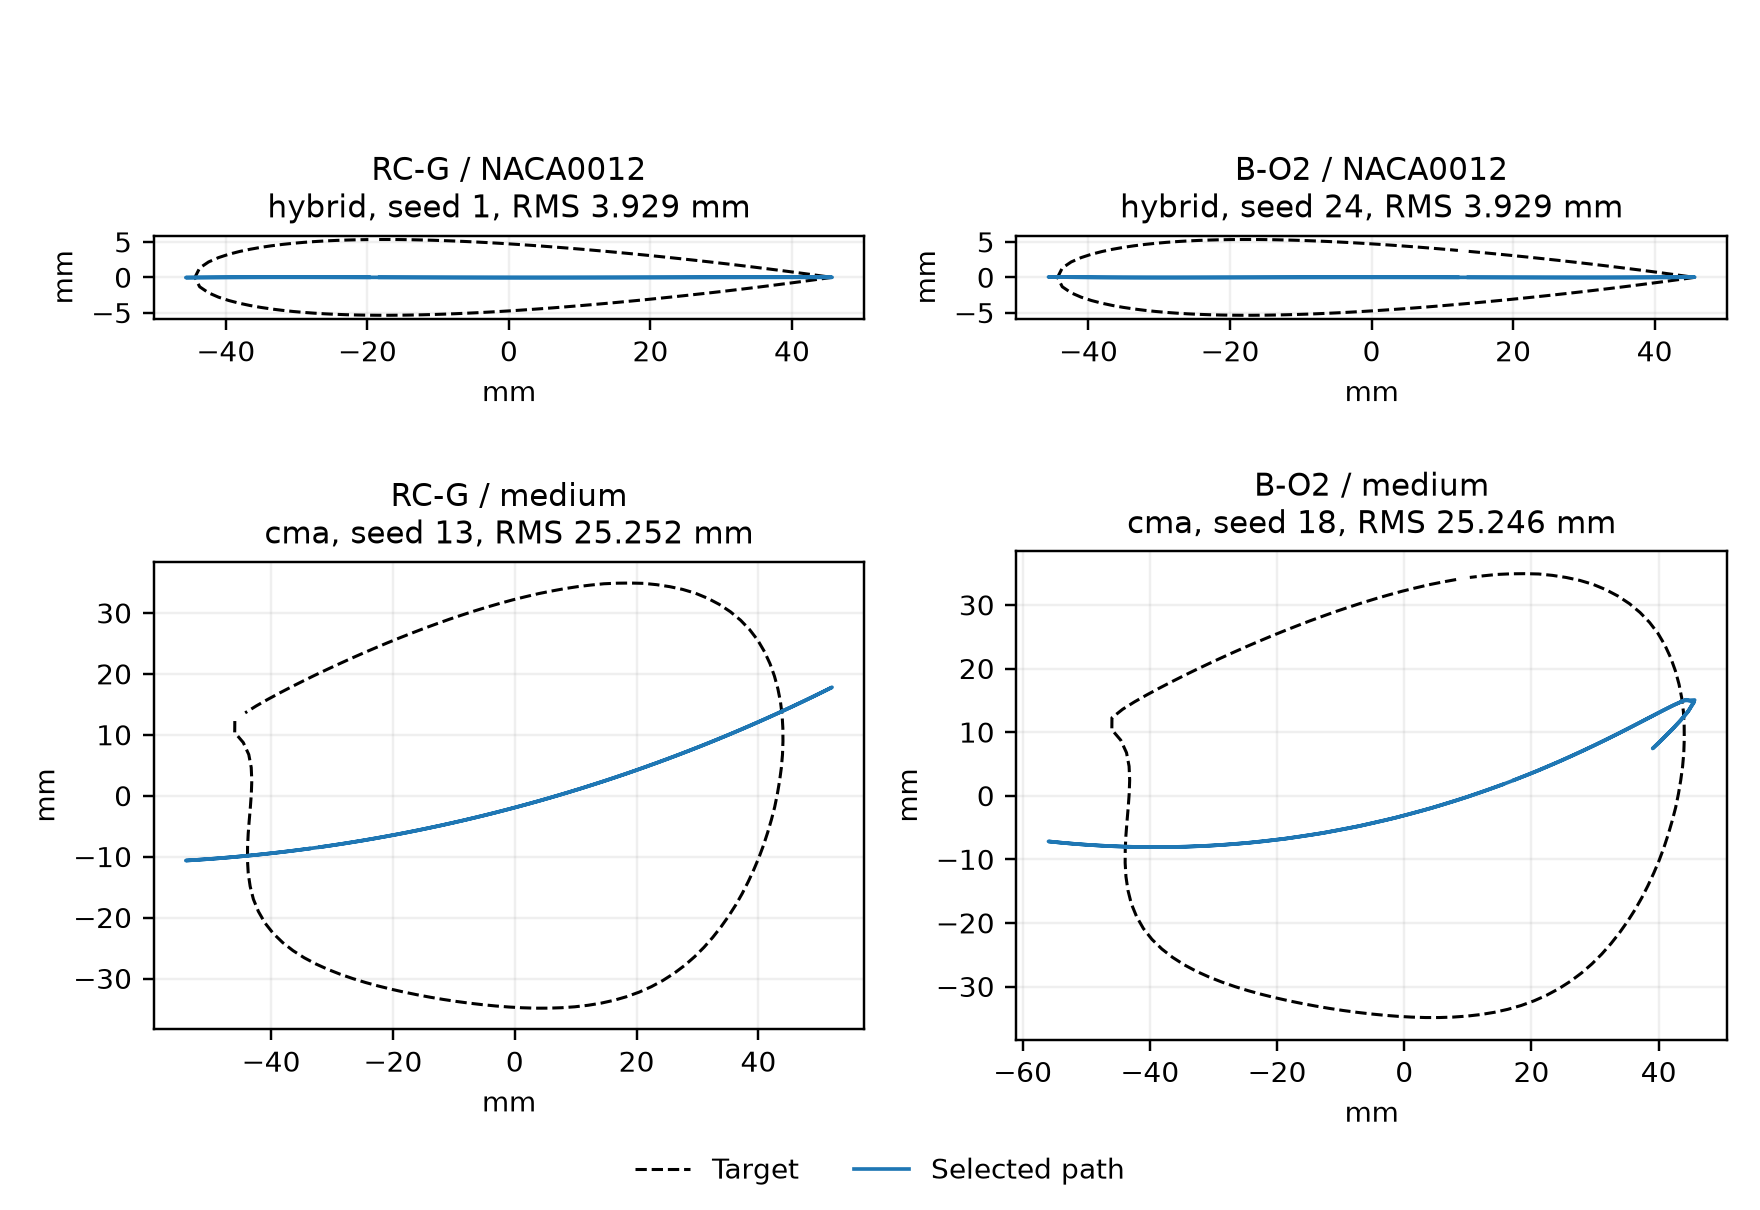
\includegraphics[width=\textwidth]{v3_model_diagnosis.png}
\caption{Retained minimum-RMS paths nearest each 30-seed median, with target and selected vector aligned at the search resolution. The supplement supplies seed IDs, actual parameter vectors and coordinates. Similar poor-fitting shapes can yield clustered RMS values without a fabricated error. The figure shows selected curve geometry, not a dense-motion certificate.}\label{fig:v3_diagnosis}
\end{figure}

\subsection{Recovery and discretization checks}
\linelabel{rev:recovery:start}Table~\ref{tab:v2_recovery} separates a generator's identity check from an independent inverse search. The optimizer receives the target, not the generator vector; one diagnostic search per model cannot estimate a recovery probability. Table~\ref{tab:v2_resolution} holds minimum-RMS selected designs fixed at the 20\,000-call checkpoint and changes sampling resolution. These counts describe retained designs, rather than every strict candidate visited by the optimizer. Tolerance sensitivity for all 16 RMS/maximum-error threshold pairs is released by model and target in the supplement; Table~\ref{tab:v2_tolerance} reports the complete grid for CD-G under compact bounds. The two counts can differ legitimately: the M columns of Tables~\ref{tab:v2_medium} and \ref{tab:v2_mediumhard} count the retained strict candidate selected by search cost and re-checked for motion, whereas Table~\ref{tab:v2_tolerance} recomputes thresholds on the minimum-RMS selected vector alone.
\begin{table}[H]
\caption{Own-curve diagnostic: one feasible generator and one separate inverse search per model (80 000 simulator calls). Generator vectors are withheld from search. A denotes any encountered strict candidate; M denotes the retained best candidate being strict and motion-valid. The identity error is a consistency check, not optimization recovery.}
\label{tab:v2_recovery}
\centering
\small
\begin{tabular}{@{}lrrrrr@{}}
\toprule
Model & Identity RMS & Inverse RMS & Inverse max & A & M \\
\midrule
F4 & 1.0e-15 & 0.061 & 0.179 & 1 & 1 \\
SC & 1.3e-15 & 0.000 & 0.000 & 1 & 1 \\
CD-G & 1.8e-15 & 0.001 & 0.004 & 1 & 1 \\
RC-G & 0.0e+00 & 0.002 & 0.006 & 1 & 1 \\
A-O4 & 1.4e-15 & 0.037 & 0.092 & 1 & 1 \\
B-O2 & 9.6e-16 & 0.013 & 0.037 & 1 & 1 \\
C-O4 & 8.3e-16 & 0.010 & 0.020 & 1 & 1 \\
G5 & 6.5e-16 & 0.155 & 0.415 & 1 & 1 \\
\bottomrule
\end{tabular}
\end{table}

\begin{table}[H]
\caption{Selected-vector resolution sensitivity for hybrid/compact at 20 000 calls. Counts satisfy both accuracy thresholds at each resolution and sampled motion validation at 1920 intervals. Each row describes eight distinct 30-seed model cells (240 selected vectors); it is not a pooled estimate of a model recovery probability. Invalid designs retain their denominator.}
\label{tab:v2_resolution}
\centering
\small
\begin{tabular}{@{}lrrrr@{}}
\toprule
Target & Selected vectors & N=120 & N=480 & N=960 \\
\midrule
Easy & 240 & 201 & 202 & 202 \\
Medium & 240 & 5 & 5 & 5 \\
Medium-hard & 240 & 20 & 20 & 20 \\
Bernoulli & 240 & 77 & 77 & 77 \\
Rectangle & 240 & 20 & 18 & 18 \\
Asymmetric & 240 & 1 & 0 & 0 \\
NACA0012 & 240 & 181 & 181 & 181 \\
\bottomrule
\end{tabular}
\end{table}

\begin{table}[H]
\caption{Post-hoc tolerance sensitivity for CD-G under compact bounds: counts of minimum-RMS selected designs passing the stated RMS and maximum-error limits, out of 30 seeds, with the selected vector held fixed. Rows: RMS limit (mm); columns: maximum-error limit (mm). These counts are recomputed from the minimum-RMS selected vector and do not re-apply the dense motion checks; the retained strict candidate counted in the M columns of Tables~\ref{tab:v2_medium} and \ref{tab:v2_mediumhard} is selected by search cost and can be a different vector, so the entries need not equal those columns.}
\label{tab:v2_tolerance}
\centering
\small
\begin{tabular}{@{}lcccc@{}}
\toprule
& \multicolumn{4}{c}{$E_{\max}$ limit} \\ \cmidrule(lr){2-5}
RMS limit & 1 & 2 & 3 & 4 \\
\midrule
\multicolumn{5}{@{}l}{\emph{Medium}}\\
0.5 & 2 & 4 & 4 & 4 \\
1.0 & 2 & 5 & 13 & 15 \\
1.5 & 2 & 6 & 15 & 20 \\
2.0 & 2 & 6 & 15 & 20 \\
\addlinespace
\multicolumn{5}{@{}l}{\emph{Medium-hard}}\\
0.5 & 7 & 7 & 7 & 7 \\
1.0 & 7 & 20 & 21 & 21 \\
1.5 & 7 & 21 & 22 & 23 \\
2.0 & 7 & 21 & 22 & 23 \\
\bottomrule
\end{tabular}
\end{table}

All eight own-curve inverse searches recover an SMV design within 80\,000 calls; this establishes consistency only for those eight archived generator cases. Resolution sensitivity exposes a limit of coarse-grid fitting: the asymmetric target's one compact minimum-RMS success at $N=120$ is absent at $N=480$ and 960, and rounded-rectangle counts fall from 20 to 18. Thus the search-grid strict indicator is not a dense-resolution guarantee. The complete per-model records preserve these changes instead of replacing the selected vectors or discarding failures.\linelabel{rev:recovery:end}

\subsection{Penalty and transmission quality}\label{sec:penalty_results}
\linelabel{rev:penalty:start}Table~\ref{tab:v2_penalty} compares the retained designs with and without the singularity penalty under the same total limit. The relevant question is whether the soft term changes motion-valid strict recovery or the separate all-dyad transmission screen, not whether its formula assigns a positive cost near a small margin. Seed-paired changes and uncertainty are released for both indicators and RMS. Neither a favorable fitting result nor a large single-loop margin establishes adequate transmission throughout every loop.

\begin{table}[H]
\caption{Controlled singularity-penalty ablation on medium/compact, 20 000 simulator calls and 30 seeds per model. The penalized row is the compatible cumulative checkpoint of the factorial, not a new independent sample. M: retained SMV; Q: additionally all transmission angles at least 30 degrees. RMS medians in mm. Removal affects both scalar cost and the LS penalty residual.}
\label{tab:v2_penalty}
\centering
\small
\begin{tabular}{@{}lrrrrrr@{}}
\toprule
Model & M pen & Q pen & M no & Q no & RMS pen & RMS no \\
\midrule
F4 & 0 & 0 & 0 & 0 & 1.315 & 1.315 \\
SC & 0 & 0 & 0 & 0 & 1.657 & 1.659 \\
CD-G & 5 & 0 & 6 & 0 & 1.007 & 1.098 \\
RC-G & 0 & 0 & 0 & 0 & 1.396 & 1.396 \\
A-O4 & 0 & 0 & 0 & 0 & 1.375 & 1.375 \\
B-O2 & 0 & 0 & 0 & 0 & 1.853 & 1.853 \\
C-O4 & 0 & 0 & 0 & 0 & 1.277 & 1.277 \\
G5 & 0 & 0 & 0 & 0 & 1.292 & 1.281 \\
\bottomrule
\end{tabular}
\end{table}

For CD-G/medium, the penalized and unpenalized protocols give 5/30 and 6/30 retained SMV designs. Neither protocol produces a retained strict design passing the all-dyad transmission screen. All eight paired motion tests have Holm-adjusted $p=1$. This experiment supplies no evidence that the current soft penalty improves the stated motion or transmission endpoints; nonsignificance does not establish its equivalence to omission.\linelabel{rev:penalty:end}

\subsection{Quality-diversity controls}\label{sec:qd_results}
\linelabel{rev:qd_results:start}Table~\ref{tab:v2_qd} reports the corrected 30-seed component study. Every run uses the same exact total, and its strict-elite vectors are available for re-simulation in both baseline and QD arms. The component contrasts refer to this common setting; the capped hybrid baseline differs in more than niche selection, so its comparison is not attributed to MAP-Elites or surrogate guidance alone. Resolution sensitivity uses a common reference archive and is supplied with seed-level results. Counts of retained elites are not counts of independent experimental units.

\begin{table}[H]
\caption{Corrected QD comparison at exactly 40 000 simulator calls per arm/seed. M counts seeds with at least one retained strict motion-valid elite; Q adds the transmission filter. Coverage and QD-score use the same reference grid. Intervals are marginal Wilson 95 percent intervals.}
\label{tab:v2_qd}
\centering
\small
\begin{tabular}{@{}lrrrrrr@{}}
\toprule
Arm & n & M & CI & Q & Coverage & QD-score \\
\midrule
baseline & 30 & 7 & [0.12, 0.41] & 0 & 0.564 & 21.64 \\
map0\_sur0 & 30 & 3 & [0.03, 0.26] & 0 & 0.602 & 12.56 \\
map0\_sur1 & 30 & 0 & [0.00, 0.11] & 0 & 0.593 & 12.93 \\
map1\_sur0 & 30 & 9 & [0.17, 0.48] & 0 & 0.837 & 28.91 \\
map1\_sur1 & 30 & 9 & [0.17, 0.48] & 0 & 0.837 & 46.38 \\
\bottomrule
\end{tabular}
\end{table}

\begin{table}[H]
\caption{Native-grid sensitivity of the full QD arm, 30 seeds each and exactly 40 000 simulator calls per run. M counts seeds with retained SMV elites. Coverage and QD-score use one common 24-by-24 reference grid for all native resolutions.}
\label{tab:v2_grid}
\centering
\small
\begin{tabular}{@{}lrrrrr@{}}
\toprule
Grid side & n & M & CI & Coverage ref & QD-score ref \\
\midrule
12 & 30 & 6 & [0.10, 0.37] & 0.827 & 50.61 \\
18 & 30 & 6 & [0.10, 0.37] & 0.835 & 47.39 \\
24 & 30 & 9 & [0.17, 0.48] & 0.837 & 46.38 \\
36 & 30 & 5 & [0.07, 0.34] & 0.835 & 40.39 \\
\bottomrule
\end{tabular}
\end{table}

At the reference grid, full QD gives 9/30 SMV seeds against 7/30 for the capped hybrid baseline. The paired difference is 0.067 (marginal bootstrap 95\% interval $-0.167$ to 0.300), with eight QD-only and six baseline-only successes and Holm-adjusted $p=1$ across the five component/baseline contrasts. MAP-Elites with the surrogate gives 9/30 versus 0/30 without MAP-Elites, adjusted $p=0.01953$, within the controlled component design. Adding the surrogate to MAP-Elites leaves both marginal counts at 9/30, with six gains and six losses; adjusted $p=1$. Median reference-grid coverage is 0.837 for full QD and 0.564 for the capped baseline. Higher descriptor coverage is consequently not interchangeable with a demonstrated improvement in strict recovery. The four native-grid strict counts are 6, 6, 9 and 5 out of 30; none of the three paired success contrasts against grid 24 is significant after Holm adjustment.\linelabel{rev:qd_results:end}

\section{Discussion}
\linelabel{rev:discussion:start}The central distinction is between finding a close geometric curve and validating a repeatable mechanism motion. The archived SC and G5 examples show that a returned point set can fit well even when the declared rigid-link or cycle assumptions fail. The CD-G recheck shows a different limitation: a valid, repeatable cycle may still approach unfavorable transmission configurations. Reporting these indicators separately is more informative than relabeling every fitting success as a feasible design.

The revised evidence also changes the meaning of a comparison across architectures. Some legacy labels represent specialized or overlapping six-bar models rather than distinct classical families. Their success rates therefore describe the implemented equations, tracer positions and parameter boxes. Neither a favorable row nor a zero row can be transferred to all inversions of a named family. In particular, own-curve recovery is a useful consistency test but does not prove comprehensive coverage or eliminate every possible modeling defect.

A practical use of the results is to screen several explicit models under an application's actual geometric, cycle and transmission requirements, then refine and validate promising designs at the required resolution. The present pose-invariant, untimed metric does not replace fixed-placement synthesis, clearance checks, force analysis, tolerance propagation or fabrication validation. The profile comparison should be used to study bounded parameter search, not to select a collision-free package.

The additional paths and independent optimizer broaden the evidence beyond the original three-curve, one-policy study. They still do not sample the distribution of industrial tasks. The Bernoulli reference supplies a canonical mathematical path, and the NACA0012 contour supplies published engineering geometry. Neither is a measured mechanism trajectory. The target set is therefore appropriate for a reproducible computational study, while application-specific generalization requires a separate, independently sourced evaluation set. The comparison also holds the eight explicit models fixed and includes no graph-based structural synthesis baseline \cite{Fogelson2023}; benchmarking against methods that search the space of linkage structures directly remains open work.

QD is assessed as a policy with explicit descriptor choices and a matched total, rather than a guaranteed source of better mechanisms. Niche occupancy depends on the descriptor ranges, reference grid and clipping. The component experiment controls the named factors, but findings remain conditional on its mutation/refinement allocation and shared-archive convention. Thirty seeds narrow uncertainty relative to the original fifteen without making small differences easy to resolve. A nonsignificant contrast is reported with its interval and is not evidence of equal policies.\linelabel{rev:discussion:end}

\section{Conclusions}
\linelabel{rev:conclusions:start}We present a corrected, reproducible comparison of eight explicitly defined planar kinematic models. A reconstruction of their graphs prevents legacy software names from being mistaken for a complete catalog of classical mechanism families. Correcting the SC geometry and the G5 one-turn cycle requirement prevents geometric fitting outputs from being counted automatically as mechanically valid path generators. Full-dyad transmission checks further separate accuracy from design quality.

The release provides \VTwoRuns{} model-level fixed-budget searches, \VTwoQDRuns{} exact-budget multi-model policy runs, separate repeated batches and own-curve recovery tests. Target, profile and cumulative budget are varied explicitly; an independent optimizer and additional paths test the dependence on search and geometry. The conclusions concern recoverability under these stated conditions. They do not establish intrinsic family rankings, industrial readiness, equivalence from nonsignificant tests or the impossibility of unobserved solutions.\linelabel{rev:conclusions:end}

\appendixtitles{yes}
\appendixstart
\appendix
\section{Complete effective parameter bounds}\label{app:bounds}
\linelabel{rev:bounds:start}The table lists every stored variable and both effective boxes after applying the profile. Angular variables are in radians, $q$ and $\rho$ are dimensionless, and the other quantities are in millimeters. G5 uses the six stated discrete ratios within the stored interval. SC's $x_0$ is a redundant translation under this metric. In the six-bar models, $C$ is the auxiliary point that carries the second dyad (fixed to coupler $AB$ in CD-G and C-O4, fixed to rocker $BO_4$ in RC-G, coincident with $A$ in A-O4 and with $B$ in B-O2), $D$ is the moving joint of the second dyad $C$--$D$--$G$, and $G$ is its ground pivot ($G=O_4$ in C-O4 and A-O4; $G=O_2$ in B-O2). In Equation~(2), $\mathbf u_{AB}$ is the unit vector from $A$ toward $B$ and $\mathbf v_{AB}$ is its 90-degree counterclockwise rotation; the tracer offsets \texttt{pu} and \texttt{pv} are measured along, and perpendicular to, the second-dyad link that carries the tracer. These bounds describe parameter search and impose no global occupied envelope.\linelabel{rev:bounds:end}
\small
\begin{longtable}{@{}llrrrr@{}}
\caption{Complete effective bounds in the revised experiments.}\label{tab:v2_bounds}\\
\toprule Model & Variable & Compact lower & Upper & Relaxed lower & Upper \\ \midrule\endfirsthead
\toprule Model & Variable & Compact lower & Upper & Relaxed lower & Upper \\ \midrule\endhead
F4 & \texttt{L1} & 35 & 150 & 35 & 234 \\
F4 & \texttt{L2} & 12 & 90 & 12 & 156 \\
F4 & \texttt{L3} & 20 & 165 & 20 & 260 \\
F4 & \texttt{L4} & 20 & 165 & 20 & 260 \\
F4 & \texttt{rP} & 0 & 150 & 0 & 286 \\
F4 & \texttt{phiP} & $-\pi$ & $\pi$ & $-\pi$ & $\pi$ \\
\addlinespace
SC & \texttt{r} & 8 & 80 & 8 & 156 \\
SC & \texttt{l} & 25 & 180 & 25 & 260 \\
SC & \texttt{q} & -0.3 & 1.35 & -0.3 & 1.35 \\
SC & \texttt{h} & -60 & 60 & -100 & 100 \\
SC & \texttt{x0} & -30 & 60 & -70 & 100 \\
\addlinespace
CD-G & \texttt{L0} & 35 & 160 & 35 & 234 \\
CD-G & \texttt{L2} & 12 & 95 & 12 & 156 \\
CD-G & \texttt{L3} & 20 & 180 & 20 & 260 \\
CD-G & \texttt{L4} & 20 & 180 & 20 & 260 \\
CD-G & \texttt{r\_c} & 0 & 150 & 0 & 286 \\
CD-G & \texttt{phi\_c} & $-\pi$ & $\pi$ & $-\pi$ & $\pi$ \\
CD-G & \texttt{gx} & -40 & 210 & -100 & 325 \\
CD-G & \texttt{gy} & -90 & 90 & -182 & 182 \\
CD-G & \texttt{L5} & 20 & 180 & 20 & 260 \\
CD-G & \texttt{L6} & 20 & 180 & 20 & 260 \\
CD-G & \texttt{pu} & -50 & 180 & -143 & 286 \\
CD-G & \texttt{pv} & -80 & 80 & -156 & 156 \\
\addlinespace
RC-G & \texttt{L0} & 35 & 160 & 35 & 234 \\
RC-G & \texttt{L2} & 12 & 95 & 12 & 156 \\
RC-G & \texttt{L3} & 20 & 180 & 20 & 260 \\
RC-G & \texttt{L4} & 20 & 180 & 20 & 260 \\
RC-G & \texttt{r\_c} & 0 & 150 & 0 & 286 \\
RC-G & \texttt{phi\_c} & $-\pi$ & $\pi$ & $-\pi$ & $\pi$ \\
RC-G & \texttt{gx} & -40 & 210 & -100 & 325 \\
RC-G & \texttt{gy} & -90 & 90 & -182 & 182 \\
RC-G & \texttt{L5} & 20 & 180 & 20 & 260 \\
RC-G & \texttt{L6} & 20 & 180 & 20 & 260 \\
RC-G & \texttt{pu} & -50 & 180 & -143 & 286 \\
RC-G & \texttt{pv} & -80 & 80 & -156 & 156 \\
\addlinespace
A-O4 & \texttt{L0} & 35 & 160 & 35 & 234 \\
A-O4 & \texttt{L2} & 12 & 95 & 12 & 156 \\
A-O4 & \texttt{L3} & 20 & 180 & 20 & 260 \\
A-O4 & \texttt{L4} & 20 & 180 & 20 & 260 \\
A-O4 & \texttt{L5} & 20 & 180 & 20 & 260 \\
A-O4 & \texttt{L6} & 20 & 180 & 20 & 260 \\
A-O4 & \texttt{pu} & -50 & 180 & -143 & 286 \\
A-O4 & \texttt{pv} & -80 & 80 & -156 & 156 \\
\addlinespace
B-O2 & \texttt{L0} & 35 & 160 & 35 & 234 \\
B-O2 & \texttt{L2} & 12 & 95 & 12 & 156 \\
B-O2 & \texttt{L3} & 20 & 180 & 20 & 260 \\
B-O2 & \texttt{L4} & 20 & 180 & 20 & 260 \\
B-O2 & \texttt{L5} & 20 & 180 & 20 & 260 \\
B-O2 & \texttt{L6} & 20 & 180 & 20 & 260 \\
B-O2 & \texttt{pu} & -50 & 180 & -143 & 286 \\
B-O2 & \texttt{pv} & -80 & 80 & -156 & 156 \\
\addlinespace
C-O4 & \texttt{L0} & 35 & 160 & 35 & 234 \\
C-O4 & \texttt{L2} & 12 & 95 & 12 & 156 \\
C-O4 & \texttt{L3} & 20 & 180 & 20 & 260 \\
C-O4 & \texttt{L4} & 20 & 180 & 20 & 260 \\
C-O4 & \texttt{r\_c} & 0 & 150 & 0 & 286 \\
C-O4 & \texttt{phi\_c} & $-\pi$ & $\pi$ & $-\pi$ & $\pi$ \\
C-O4 & \texttt{L5} & 20 & 180 & 20 & 260 \\
C-O4 & \texttt{L6} & 20 & 180 & 20 & 260 \\
C-O4 & \texttt{pu} & -30 & 180 & -143 & 286 \\
C-O4 & \texttt{pv} & -70 & 70 & -156 & 156 \\
\addlinespace
G5 & \texttt{L0} & 35 & 160 & 35 & 234 \\
G5 & \texttt{L2} & 10 & 95 & 10 & 156 \\
G5 & \texttt{L4} & 10 & 95 & 10 & 260 \\
G5 & \texttt{L3} & 20 & 180 & 20 & 260 \\
G5 & \texttt{L5} & 20 & 180 & 20 & 260 \\
G5 & \texttt{ratio} & -3 & 3 & -3 & 3 \\
G5 & \texttt{phase} & $-\pi$ & $\pi$ & $-\pi$ & $\pi$ \\
G5 & \texttt{r\_p} & 0 & 150 & 0 & 286 \\
G5 & \texttt{phi\_p} & $-\pi$ & $\pi$ & $-\pi$ & $\pi$ \\
\addlinespace
\bottomrule\end{longtable}\normalsize

\section{Descriptive sampled point envelopes}\label{app:envelopes}
\linelabel{rev:envelopes:start}The following statistics use minimum-RMS selected vectors, including designs that fail the fitting thresholds. They describe only the vectors that close on the dense grid; the accompanying valid counts expose this conditioning. Neither profile is redefined as a geometric packaging constraint.\linelabel{rev:envelopes:end}
\begin{table}[H]
\caption{Sampled point envelopes of minimum-RMS selected designs at 20 000 calls. M/MH: medium/medium-hard; C/R: compact/relaxed. Valid counts are out of 30 and refer to geometric closure on the 1920-interval grid. Area is in thousands of square millimeters; radius is in millimeters. Medians exclude failed dense closures and keep their counts visible. These descriptive point envelopes do not model body thickness or collisions.}
\label{tab:v3_envelopes}
\centering
\small
\begin{tabular}{@{}llrrrrrr@{}}
\toprule
Target & Model & Valid C & Valid R & Area C & Area R & Radius C & Radius R \\
\midrule
M & F4 & 30 & 30 & 12.33 & 36.17 & 81.7 & 220.7 \\
M & SC & 30 & 30 & 11.14 & 11.12 & 75.1 & 75.2 \\
M & CD-G & 23 & 25 & 47.24 & 98.04 & 187.7 & 244.0 \\
M & RC-G & 25 & 15 & 58.34 & 115.75 & 215.5 & 297.7 \\
M & A-O4 & 30 & 30 & 37.29 & 50.20 & 204.7 & 237.9 \\
M & B-O2 & 30 & 30 & 31.19 & 103.16 & 102.9 & 207.4 \\
M & C-O4 & 30 & 30 & 41.92 & 73.79 & 179.4 & 241.0 \\
M & G5 & 19 & 21 & 22.96 & 45.95 & 148.0 & 230.1 \\
MH & F4 & 30 & 30 & 18.33 & 38.38 & 109.1 & 221.4 \\
MH & SC & 30 & 30 & 11.36 & 11.32 & 87.0 & 86.9 \\
MH & CD-G & 27 & 28 & 46.04 & 122.92 & 182.0 & 280.2 \\
MH & RC-G & 26 & 26 & 63.44 & 133.50 & 183.2 & 264.4 \\
MH & A-O4 & 30 & 30 & 33.84 & 62.47 & 184.2 & 216.5 \\
MH & B-O2 & 24 & 28 & 59.65 & 120.51 & 147.6 & 236.3 \\
MH & C-O4 & 30 & 30 & 43.82 & 85.72 & 192.9 & 253.2 \\
MH & G5 & 24 & 25 & 38.88 & 77.14 & 171.0 & 268.8 \\
\bottomrule
\end{tabular}
\end{table}


\supplementary{Versioned corrected engine, complete effective bounds, original and revised campaign records, target formulas, retained vectors, validation and statistical scripts, and a SHA-256 manifest are provided with the supplementary archive.}

%%%%%%%%%%%%%%%%%%%%%%%%%%%%%%%%%%%%%%%%%%%%%%%%%%%%%%%%%%%%
\authorcontributions{Conceptualization, R.S.F., C.P.P.M. and D.A.H.;
methodology, R.S.F., C.P.P.M. and D.A.H.; software, R.S.F., C.P.P.M.
and D.A.H.; validation, R.S.F., C.P.P.M. and D.A.H.; formal analysis,
R.S.F., C.P.P.M. and D.A.H.; investigation, R.S.F., C.P.P.M. and
D.A.H.; data curation, R.S.F., C.P.P.M. and D.A.H.; writing---original
draft preparation, R.S.F., C.P.P.M. and D.A.H.; writing---review and
editing, R.S.F., C.P.P.M. and D.A.H. }

\funding{This research received no external funding.}

\institutionalreview{Not applicable.}

\informedconsent{Not applicable.}

\dataavailability{The corrected simulation outputs, source code, retained vectors, validation results and evidence index are available in the revision branch at \url{https://github.com/romusan/fef-graph-capability-benchmark/tree/revision/applsci-4642776}. The revision includes a SHA-256 file manifest and reproduction instructions. Historical and corrected protocols are identified separately. The same scientific evidence accompanies the supplementary archive.}
\acknowledgments{\linelabel{rev:ack:start}We acknowledge Universidad Militar Nueva Granada and
Universidad ECCI for their institutional support and for providing the
academic environment and computational resources that made this work
possible. During the preparation of this manuscript, the authors used
Anthropic Claude Opus for language editing and for the construction of
the analysis and experiment code, and OpenAI Codex for editorial
adaptation and for constructing audit scripts to cross-check archived
outputs; the peer-review revision used Kimi and OpenAI Codex as AI coding
assistants to re-analyze archived data (statistical reanalysis,
post-hoc kinematic checks, and recovery tests), under full author
supervision. The authors remain responsible for verifying the analyses, reviewing the text and approving the submitted version.\linelabel{rev:ack:end}}
\conflictsofinterest{The authors declare no conflict of interest.}

%%%%%%%%%%%%%%%%%%%%%%%%%%%%%%%%%%%%%%%%%%%%%%%%%%%%%%%%%%%%
\abbreviations{Abbreviations}{
The following abbreviations are used in this manuscript:\\

\noindent
\begin{tabular}{@{}ll}
RMS & Root mean square\\
QD & Quality diversity\\
DE & Differential evolution\\
CI & Confidence interval\\
CMA-ES & Covariance matrix adaptation evolution strategy\\
MAP-Elites & Multi-dimensional archive of phenotypic elites\\
SMV & Strict motion-valid
\end{tabular}

\noindent
Model identifiers (F4, SC, CD-G, RC-G, A-O4, B-O2, C-O4, G5) are defined in Table~\ref{tab:v2_models}.
}

%%%%%%%%%%%%%%%%%%%%%%%%%%%%%%%%%%%%%%%%%%%%%%%%%%%%%%%%%%%%
\begin{adjustwidth}{-\extralength}{0cm}
\reftitle{References}

\begin{thebibliography}{999}
\bibitem{Freudenstein1954}
Freudenstein, F. An analytical approach to the design of four-link
mechanisms. \textit{Trans. ASME} \textbf{1954}, \textit{76},
483--489. \url{https://doi.org/10.1115/1.4014881}.
% Reference 3

\bibitem{McCarthy2010}
McCarthy, J.M.; Soh, G.S. \textit{Geometric Design of Linkages}, 2nd
ed.; Springer: New York, NY, USA, 2010.
% Reference 8

\bibitem{Storn1997}
Storn, R.; Price, K. Differential evolution---A simple and efficient
heuristic for global optimization over continuous spaces. \textit{J.
Glob. Optim.} \textbf{1997}, \textit{11}, 341--359.
\url{https://doi.org/10.1023/A:1008202821328}.
% Reference 14

\bibitem{Kang2022}
Kang, Y.H.; Lin, J.W.; You, W.C. Comparative study on the synthesis
of path-generating four-bar linkages using metaheuristic optimization
algorithms. \textit{Appl. Sci.} \textbf{2022}, \textit{12}, 7368.
\url{https://doi.org/10.3390/app12157368}.
% Reference 19

\bibitem{Winyangkul2026}
Winyangkul, S.; Alfouneh, M.; Sleesongsom, S. Four-bar linkage path
generation problems using a new TLBO and optimum path repairing
technique. \textit{Biomimetics} \textbf{2026}, \textit{11}, 160.
\url{https://doi.org/10.3390/biomimetics11030160}.
% Reference 20

\bibitem{Soh2008}
Soh, G.S.; McCarthy, J.M. The synthesis of six-bar linkages as
constrained planar 3R chains. \textit{Mech. Mach. Theory}
\textbf{2008}, \textit{43}, 160--170.
\url{https://doi.org/10.1016/j.mechmachtheory.2007.02.004}.
% Reference 31

\bibitem{Plecnik2016a}
Plecnik, M.M.; McCarthy, J.M. Design of Stephenson linkages that
guide a point along a specified trajectory. \textit{Mech. Mach.
Theory} \textbf{2016}, \textit{96}, 38--51.
\url{https://doi.org/10.1016/j.mechmachtheory.2015.08.015}.
% Reference 33

\bibitem{Plecnik2016b}
Plecnik, M.M.; McCarthy, J.M. Kinematic synthesis of Stephenson III
six-bar function generators. \textit{Mech. Mach. Theory}
\textbf{2016}, \textit{97}, 112--126.
\url{https://doi.org/10.1016/j.mechmachtheory.2015.10.004}.
% Reference 34

\bibitem{Fogelson2023}
Fogelson, M.B.; Tucker, C.; Cagan, J. GCP-HOLO: Generating high-order
linkage graphs for path synthesis. \textit{J. Mech. Des.}
\textbf{2023}, \textit{145}, 073303.
\url{https://doi.org/10.1115/1.4062147}.
% Reference 39

\bibitem{Pugh2016}
Pugh, J.K.; Soros, L.B.; Stanley, K.O. Quality diversity: A new
frontier for evolutionary computation. \textit{Front. Robot. AI}
\textbf{2016}, \textit{3}, 40.
\url{https://doi.org/10.3389/frobt.2016.00040}.
% Reference 41

\bibitem{Mouret2015}
Mouret, J.-B.; Clune, J. Illuminating search spaces by mapping
elites. \textit{arXiv} \textbf{2015}, arXiv:1504.04909.
\url{https://doi.org/10.48550/arXiv.1504.04909}.
% Reference 43

\bibitem{Holm1979}
Holm, S. A simple sequentially rejective multiple test procedure.
\textit{Scand. J. Stat.} \textbf{1979}, \textit{6}, 65--70.
% Reference 44

\bibitem{Wilson1927}
Wilson, E.B. Probable inference, the law of succession, and statistical
inference. \textit{J. Am. Stat. Assoc.} \textbf{1927}, \textit{22},
209--212. \url{https://doi.org/10.1080/01621459.1927.10502953}.
% Reference 49

\bibitem{McNemar1947}
McNemar, Q. Note on the sampling error of the difference between
correlated proportions or percentages. \textit{Psychometrika}
\textbf{1947}, \textit{12}, 153--157.
\url{https://doi.org/10.1007/BF02295996}.
% Reference 50

\bibitem{Virtanen2020}
Virtanen, P.; Gommers, R.; Oliphant, T.E.; Haberland, M.; Reddy, T.;
Cournapeau, D.; Burovski, E.; Peterson, P.; Weckesser, W.; Bright,
J.; et al. SciPy 1.0: Fundamental algorithms for scientific computing
in Python. \textit{Nat. Methods} \textbf{2020}, \textit{17},
261--272. \url{https://doi.org/10.1038/s41592-019-0686-2}.
% Reference 51

\bibitem{BernoulliReference} University of St Andrews. Lemniscate of Bernoulli. MacTutor History of Mathematics. \url{https://mathshistory.st-andrews.ac.uk/Curves/Lemniscate/} (accessed on 16 October 2026).

\bibitem{NASATMR} Turbulence Modeling Resource. Two-Dimensional NACA 0012 Airfoil Validation Case. NASA-linked reference geometry. \url{https://tmbwg.github.io/turbmodels/naca0012_val.html} (accessed on 16 October 2026).

\bibitem{SciPyDE} The SciPy Community. Differential Evolution. SciPy Reference Documentation. \url{https://docs.scipy.org/doc/scipy/reference/generated/scipy.optimize.differential_evolution.html} (accessed on 16 October 2026).

\bibitem{HansenCMA} CMA-ES Developers. Pycma Documentation and Source Code, version 4.5.0. \url{https://cma-es.github.io/apidocs-pycma/} (accessed on 16 October 2026).


\end{thebibliography}

\PublishersNote{}
\end{adjustwidth}
\end{document}
